\documentclass[10pt,a4paper]{article}
\usepackage[margin=2.2cm]{geometry}
\usepackage{fontspec}
\usepackage{kotex}
\setmainfont{Apple SD Gothic Neo}
\setsansfont{Apple SD Gothic Neo}
\usepackage{amsmath,amssymb}
\usepackage{graphicx}
\usepackage{booktabs}
\usepackage{caption}
\usepackage[dvipsnames]{xcolor}
\usepackage[colorlinks=true,linkcolor=MidnightBlue,citecolor=MidnightBlue,
            urlcolor=MidnightBlue]{hyperref}
\usepackage{titlesec}
\titleformat{\section}{\large\bfseries}{\thesection}{0.6em}{}
\captionsetup{font=small,labelfont=bf}
\setlength{\parskip}{0.35em}
\setlength{\parindent}{0pt}

\usepackage{mdframed}
\newmdenv[linewidth=0.4pt,linecolor=gray!60,backgroundcolor=gray!5,
          innertopmargin=6pt,innerbottommargin=6pt,skipabove=8pt,skipbelow=8pt]{claimbox}
\newcommand{\claim}[2]{\begin{claimbox}\textbf{주장.} #1\par\smallskip
  \textcolor{gray!70}{\textbf{반증 조건.} #2}\end{claimbox}}

\title{\bfseries 한 축 위에서\\[2pt]
\large 합동 모형은 공유 기저를 안 쓴다 --- 그리고 도메인 범주가 겹쳐 있었다}
\author{월드모델 실험실 · 노트 $819 \sim 820$}
\date{2026-08-07}
\begin{document}\maketitle

\section{한 줄 둘}

\textbf{①(노트 $819$)} 사용자의 $36$축 고정 기저 물음을 모델 내부에서 쟀다 ---
챔피언 합동 적합의 도메인별 \textbf{치환 중요도 벡터}($36$축 확인 · 값$\cdot$
표시자 쌍 치환 $6$뽑기 · 자기 천장은 반-반 $6$뽑기)의 교차 코사인. 결과는
\textbf{갈래 $5$ · 정렬 없음}: 셔플 널 초과 $14/55$쌍($25\%$ --- 문턱 $50\%$
미달), 교차 중앙 $0.251$ 대 자기 천장 중앙 $0.862$. 천장이 높으니 \emph{잡음이
아니라 실제로 안 겹치는 것}이다. 내 주 예측(부분 공유)은 틀렸고, 부 예측
(아이돌 교차 최하위)은 맞았다.

\textbf{②(노트 $820$ · 사용자 ①)} ``게임-모바일 $0.66\times$바닥은 범주가
실제로 겹치는 것 아닌가''를 셌다 --- \textbf{겹친다.} 게임-모바일 $38$개
(게임의 $7.9\%$), \textbf{만화-세계애니 $838$개(세계애니의 $29\%$)}. 논문
$176$ 의 ``게임-모바일 같다''와 $819$ 의 만화-세계애니 정렬($0.795$)은
\textbf{겹침 제외 재측정 전까지 보류}한다.

\begin{figure}[t]\centering
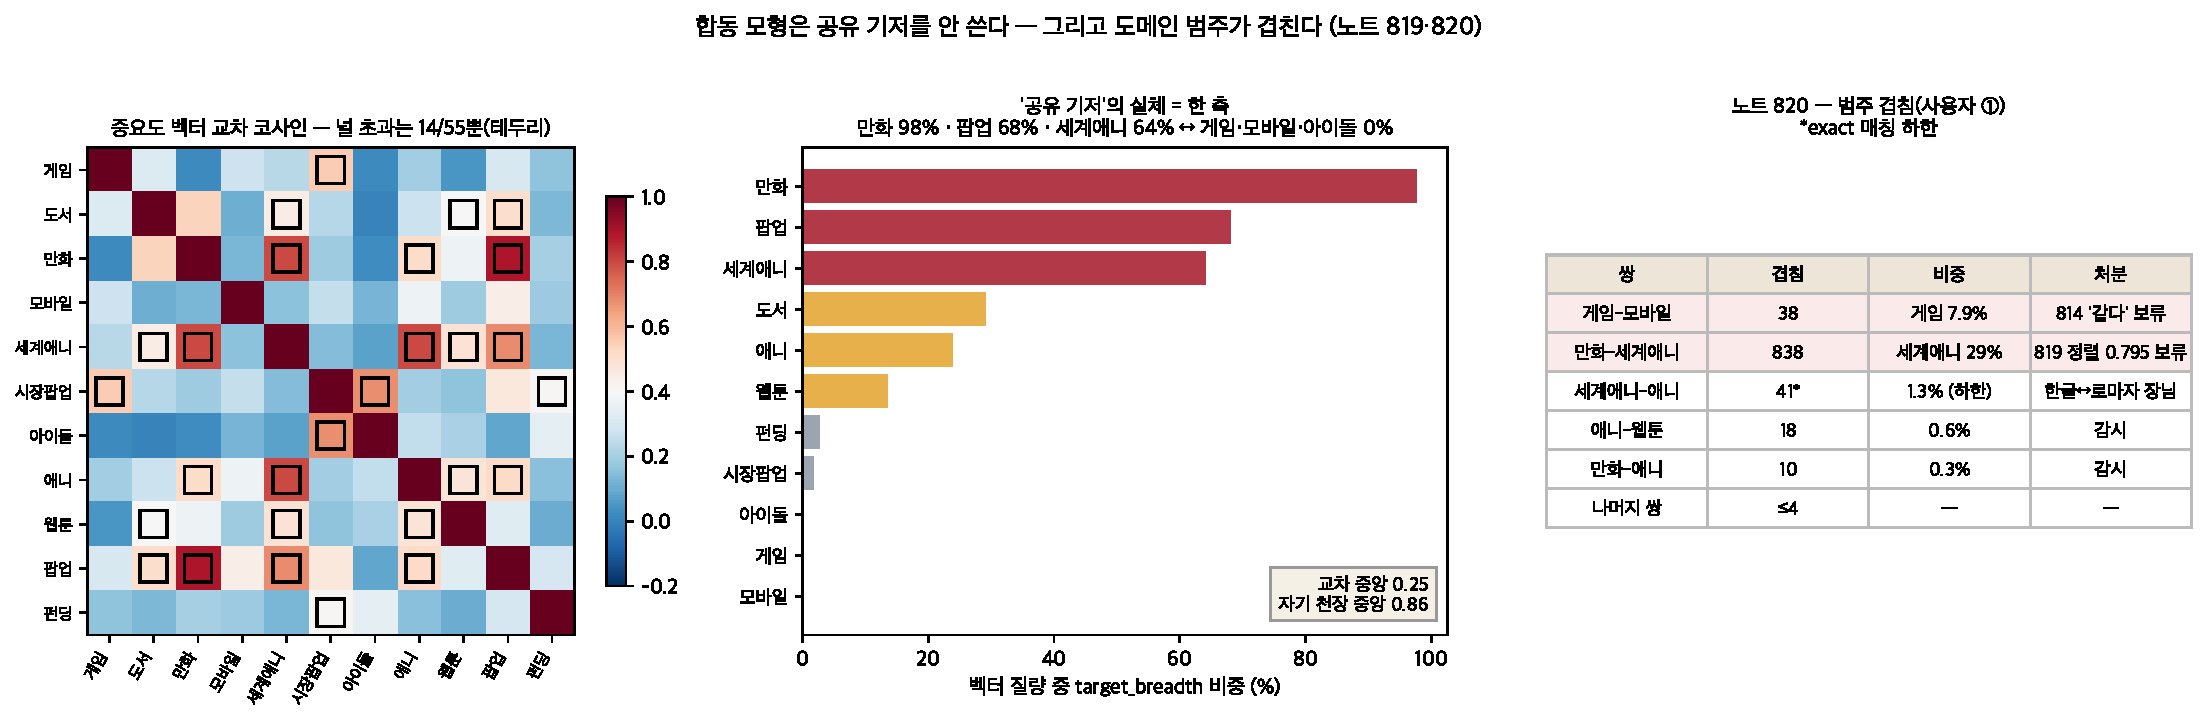
\includegraphics[width=0.99\textwidth]{figs/onaxis.pdf}
\caption{왼쪽: $11{\times}11$ 교차 코사인 --- 널 초과(테두리)는 $14$쌍뿐.
가운데: 정렬의 실체는 \textbf{target\_breadth 한 축}. 오른쪽: 범주 겹침 표.}
\end{figure}

\section{`공유 기저'의 실체는 한 축이다}

\claim{\textbf{정렬된 쌍의 코사인은 target\_breadth 혼자 든다} --- 만화-팝업
$0.883$ 중 $0.815$, 만화-세계애니 $0.795$ 중 $0.791$. 도메인 벡터의
target\_breadth 질량: 만화 $98\%$ · 팝업 $68\%$ · 세계애니 $64\%$ ↔ 게임 ·
모바일 · 아이돌 $0\%$(그들의 몸통은 goods\_scale · entry\_friction ·
venue\_prominence --- 도메인 조건부). TabPFN 이 구한 두 도메인은 \textbf{서로
다른 이유}로 소외였다: 아이돌은 벡터가 안정한데 방향이 다르고(교차 최하위
$0.181$), 시장팝업은 벡터 자체가 불안정(자기 천장 $0.210$ --- 유일한 $0.5$
미만). $818$(자료 층)과 같은 그림이다 --- \textbf{이 판의 `파운데이션'은 넓은
공유 기저가 아니라 한 줌의 공유 $+$ 도메인 조건부 몸통이고, 합동의 이득은 기저
공유가 아니라 표본 공유(정칙화)로 읽는 것이 맞다.}}
{치환 중요도는 상관 축 사이에서 몫을 가른다 --- 도메인마다 축 상관구조가
다르면 같은 함수라도 벡터가 갈라질 수 있다(과대 판정 위험). KOBIS 합류 시
상관-무리 단위 조건부 치환으로 $1$회 재검, 그때도 $25\%$ 안팎이면 확정.
그리고 $819$ 의 만화-세계애니 정렬 자체가 $820$ 의 겹침 오염 후보다.}

\section{다음 문 --- 사용자 제안 순서대로}

① 겹침 제외 재측정($176$ 세 쌍 $+$ $819$ 정렬 쌍 · 애니 계열은 로마자$\leftrightarrow$
한글 매칭 먼저) ② \textbf{경쟁 베이스라인}(시간 갈림 · 최근 작품에서 원작
순위 그대로 / 직전 분기 평균 / $36$축 릿지 --- $\rho 0.30$ 의 존폐, T$1$ 최우선
등록 · \emph{이것 전에 판권 문 안 두드림}) ③ 거리 자 교체(RMSE 는 다봉성에
둔감 --- 감쇠-이중피크 재검) ④ 드리프트율을 $\tau$ · 진폭에 이은 셋째 도메인
모수로. 판 $\rho$ $0.4689$ 그대로.

\end{document}
